% arara: lualatex: {
% arara: --> shell: no,
% arara: --> draft: yes,
% arara: --> interaction: batchmode
% arara: --> }
% arara: bibtex
% arara: lualatex: {
% arara: --> shell: no,
% arara: --> draft: no,
% arara: --> interaction: batchmode
% arara: --> }
% arara: lualatex: {
% arara: --> shell: no,
% arara: --> draft: no,
% arara: --> interaction: batchmode
% arara: --> }
% arara: clean: {
% arara: --> extensions:
% arara: --> ['aux','bbl','blg','lof','log','lot','out','toc']      
% arara: --> }
\RequirePackage[svgnames]{xcolor}
\documentclass[
  11pt,
  a4paper,
  oneside,
  english,
  spanish
]{TesisUNI}

\usepackage[natbibapa]{apacite} %Agregar formato de citación APA
\bibliographystyle{apacite}
\setlength{\bibsep}{5pt plus 0.3ex} %Espaciamiento en la bibliografía
\setcounter{secnumdepth}{3} %Numera los subsubsecciones
% \usepackage[T1]{fontenc}
\usepackage[spanish,es-tabla]{babel} %reemplaza "cuadro" por "tabla"
\decimalpoint % Cambia coma por punto
\usepackage{mathptmx}
% \usepackage[cmintegrals]{newtxmath}
\usepackage{layouts} % Saber ancho de hoja.
\usepackage{fontspec}
\usepackage[ISO]{diffcoeff}
\usepackage{amsthm}
\usepackage{mathtools}
% \usepackage{bm}
\usepackage{amssymb}
\let\mathbbalt\mathbb
\usepackage{graphicx}
\usepackage{changepage} % Agregar identación
\setmainfont{Arial}
\usepackage{setspace}
\usepackage[left=4 cm,right=3 cm,top=3 cm,bottom=3.5 cm]{geometry}
\usepackage{fancyhdr} % Encabezado y Pie de página (1)
\pagestyle{fancy} % Encabezado y Pie de página (2)
\usepackage{lipsum} % Crear texto RAMDOM
\renewcommand{\labelitemi}{$\bullet$} % Circulos para viñetas
\usepackage{titlesec} % Titulos de SECCIONES
\usepackage{tocloft} % Titulos de ÍNDICES
\usepackage[colorlinks=true,linkcolor=negro,citecolor = negro]{hyperref}
\usepackage[mathbf=sym]{unicode-math} % Mantener fuentes matemáticas
\removenolimits{\int} % https://tex.stackexchange.com/a/103925
\let\mathbb\mathbbalt
\makeatletter  % Comando para REDUCIR ERRORES
\usepackage{multirow} % Agregar TABLAS 
\usepackage{array} % Dar formato a las TABLAS
\usepackage{subcaption} % Insertar SubImagenes
\usepackage{tikz} % Diagrama de Flujo
\usetikzlibrary{calc,positioning,shapes.geometric,shapes.symbols,shapes.misc}

% Insertar formas para diagramas de flujo
\tikzstyle{startstop} = [rectangle, rounded corners, minimum width=3cm, minimum height=0.5cm,text centered, draw=black]
\tikzstyle{io} = [trapezium, trapezium left angle=70, trapezium right angle=110, minimum width=3cm, minimum height=0.5cm, text centered, text width=3cm, draw=black]
\tikzstyle{process} = [rectangle, minimum width=3cm, minimum height=0.5cm, text centered, text width=4cm, draw=black]
\tikzstyle{decision} = [diamond, minimum width=3cm, minimum height=0.5cm, text centered, draw=black]
\tikzstyle{loop} = [chamfered rectangle,chamfered rectangle xsep=2cm,draw=black]
\tikzstyle{arrow} = [->,>=stealth]
\tikzstyle{line}=[draw]

\usepackage{listings}
\usepackage{color}

\AtBeginDocument{\let\setminus\smallsetminus}
\DeclareMathAlphabet{\mathcal}{OMS}{cmsy}{m}{n}

%New colors defined below
\definecolor{codegreen}{rgb}{0,0.6,0}
\definecolor{codegray}{rgb}{0.5,0.5,0.5}
\definecolor{codepurple}{rgb}{0.2,0,1}
\definecolor{codeRojo}{rgb}{0.7,0,0.3}
\definecolor{backcolour}{rgb}{1.0, 1.0, 1.0}

%Code listing style named "mystyle"
\lstdefinestyle{mystyle}{
  backgroundcolor=\color{backcolour},
  commentstyle=\color{codegreen},
  keywordstyle=\color{codeRojo},
  numberstyle=\tiny\color{codegray},
  stringstyle=\color{codepurple},
  basicstyle=\footnotesize,
  breakatwhitespace=false,
  breaklines=true,
  captionpos=b,
  keepspaces=true,
  numbers=left,
  numbersep=5pt,
  showspaces=false,
  showstringspaces=false,
  showtabs=false,
  tabsize=2
}

%"mystyle" code listing set
\lstset{style=mystyle}

\newenvironment{MyFont}{\fontfamily{ugm}\selectfont}{\par}

\usepackage{changepage} % Agregar espacio a Listing

% Centrado del título del ÍNDICE / LISTA DE FIGURAS / LISTA DE CUADROS

\renewcommand{\cfttoctitlefont}{\hfill \normalfont\normalsize\bfseries}
\renewcommand{\cftaftertoctitle}{\hfill}

\renewcommand{\cftlottitlefont}{\hfill\normalfont\normalsize\bfseries}
\renewcommand{\cftafterlottitle}{\hfill}

\renewcommand{\cftloftitlefont}{\hfill\normalfont\normalsize\bfseries}
\renewcommand{\cftafterloftitle}{\hfill}

% Formato de los CAPÍTULOS, SECCIONES Y SUBSECCIONES
\titleformat{\chapter}[block]{\normalfont\normalsize\bfseries}{CAPÍTULO \thechapter:}{0.5em}{\normalsize}
\titlespacing*{\chapter}{0pt}{-10 pt}{5pt}

\titleformat{\section}[block]{\normalfont\normalsize}{\thesection}{0.5em}{\normalsize}
\titlespacing*{\section}{0pt}{10 pt}{5 pt}

\titleformat{\subsection}[block]{\normalfont\normalsize}{\thesubsection}{0.5em}{\normalsize}
\titlespacing*{\subsection}{0pt}{10 pt}{5 pt}

\titleformat{\subsubsection}[block]{\normalfont\normalsize}{\thesubsubsection}{0.5em}{\normalsize}
\titlespacing*{\subsubsection}{0pt}{10 pt}{5 pt}

% Espaciado entre PÁRRAFOS y SANGRÍA
\setlength{\parskip}{5 pt}
\setlength{\parindent}{0cm}

% Dar formato a las TABLAS
\newcolumntype{M}[1]{>{\centering\arraybackslash}m{#1}}
\newcolumntype{L}[1]{>{\raggedright\arraybackslash}m{#1}}
\newcolumntype{R}[1]{>{\raggedleft\arraybackslash}m{#1}}
\newcolumntype{N}{@{}m{0pt}@{}}
\renewcommand{\arraystretch}{1.25}

% Cambiar titulo de bibliografía
\addto\captionsspanish{\renewcommand{\bibname}{\centering REFERENCIAS BIBLIOGRÁFICAS}}

% Posicionamiento vertical de TOC, LOT and LOF

\setlength{\cftbeforelottitleskip}{1pt}
\renewcommand{\cftafterlottitleskip}{12pt}

\setlength{\cftbeforeloftitleskip}{1pt}
\renewcommand{\cftafterloftitleskip}{12pt}

\setlength{\cftbeforetoctitleskip}{16pt}
\renewcommand{\cftaftertoctitleskip}{12 pt}

% Cambiando las etiquetas de las FIGURAS y TABLAS (Caption y autoref)
\addto\captionsspanish{\renewcommand{\figurename}{\footnotesize FIGURA N°}}
\addto\extrasspanish{\def\figureautorefname{Figura N°}}

\addto\captionsspanish{\renewcommand{\tablename}{\footnotesize TABLA N°}}
\addto\extrasspanish{\def\tableautorefname{Tabla N°}}

% Espaciamiento dentro del índice

\setlength{\cftbeforechapskip}{2mm}
\renewcommand\cftchapafterpnum{\vskip6pt}
\renewcommand\cftsecafterpnum{\vskip5pt}
\renewcommand\cftsubsecafterpnum{\vskip5pt}

%Agregar la palabra CAPITULO al TOC, FIGURA a LOF y TABLA al LOT

\renewcommand{\cftchappresnum}{CAPÍTULO}
\renewcommand{\cftchapaftersnum}{:}
\renewcommand{\cftchapnumwidth}{7em}

\renewcommand{\cftfigpresnum}{Figura N°}
%\renewcommand{\cftfigaftersnum}{:}
\renewcommand{\cftfignumwidth}{6.85 em}

\renewcommand{\cfttabpresnum}{Tabla N°}
%\renewcommand{\cftfigaftersnum}{:}
\renewcommand{\cfttabnumwidth}{6.5 em}

%Definición de COLORES
\definecolor{granate}{RGB}{113,22,16}
\definecolor{gris}{RGB}{154,153,157}
\definecolor{arena}{RGB}{230,217,170}
\definecolor{azul}{rgb}{0.03,0.15,0.4}
\definecolor{negro}{rgb}{0,0,0}

%Cambiando a Números Romanos los Capítulos
\renewcommand{\thechapter}{\Roman{chapter}}
\renewcommand{\theequation}{\arabic{chapter}.\arabic{equation}}
\renewcommand{\thesection}{\arabic{chapter}.\arabic{section}}
\renewcommand{\thetable}{\arabic{chapter}.\arabic{table}}
\renewcommand{\thefigure}{\arabic{chapter}.\arabic{figure}}

\providecommand{\averageconcentration}{\overline{u}\left(x,t\right)}
\providecommand{\inner}[2]{\left\langle #1, #2 \right\rangle}
\difdef{c}{L}{op-symbol=\mathop{}\!\mathbin\bigtriangleup}
\difdef{c}{A}{op-symbol=\mathop{}\!\mathbin\Box}


\theoremstyle{definition}
\newtheorem{theorem}{Teorema}
\newtheorem{definition}{Definición}
\newtheorem{example}{Ejemplo}
\newtheorem{proposition}{Proposición}

% Escribir los INFORMACIÓN PERSONAL Y DEL TRABAJO

%Autor para PIE DE PÁGINA (Respetar mayusculas y minisculas)
\author{Carlos Alonso Aznarán Laos}

%Autor para CARÁTULA (Siempre en mayuscula y sin saltos de linea)
\authorcaratula{CARLOS ALONSO AZNARÁN LAOS}

%Título en para el PIE DE PÁGINA (Agregar salto de línea de ser necesario)
% La selección de un esquema Upwind y Lax-Wendroff para la solución numérica de la ecuación advección-difusión
% Minimización del error en los métodos Upwind y Lax-Wendroff para la solución numérica de la ecuación advección-difusión % Evolutivos
% Estimación del Error en los Esquemas Upwind y Lax-Wendroff de la ecuación de Advección-Difusión lineal
\title{Estimación del Error en los Esquemas de Alta Resolulución de la ecuación de Advección-Difusión lineal}
%Título para CARÁTULA (Siempre en mayuscula y sin saltos de linea)
\titlecaratula{ESTIMACIÓN DEL ERROR EN LOS ESQUEMAS DE ALTA RESOLUCIÓN DE LA ECUACIÓN DE ADVECCIÓN-DIFUSIÓN LINEAL} % EVOLUTIVOS
%Nombre de la FACULTAD (Siempre en mayuscula)
\facultad{FACULTAD DE CIENCIAS}

%Para obtener el título profesional de ... (Siempre en mayúscula)
\grado{LICENCIADO EN MATEMÁTICA}

%Asesor para CARÁTULA (Siempre en mayuscula y sin saltos de linea)
\asesor{DR. JONATHAN ALFREDO MUNGUÍA LA COTERA}

% Año para la CARÁTULA
\yyearr{2024}

\begin{document}

\renewcommand{\BOthers}[1]{et al.\hbox{}} %Agregar et al.
\onehalfspacing 	% Interlineado 1.5
\noindent			% Sin sangría

% Parte inicial de la tesis

\frontmatter

\begin{titlepage}
	\begin{center}
		\vspace*{2 mm}
		{\LARGE \textbf{UNIVERSIDAD NACIONAL DE INGENIERÍA}}\\
		\vspace{5 mm}
		{\LARGE \textbf{\@facultad}}\\
		\vspace{6.5 mm}
		\begin{figure}[h]
			\centering
			
\includegraphics[scale=1]{E_IMAGENES/0_Caratula/UNI_LOGO1.pdf}
		\end{figure}
		\vspace{1 mm}
		{\Large \textbf{PROYECTO DE TESIS I} }\\
		\vspace{5 mm}

		\onehalfspacing  % Espaciamiento 1.5
		{\Large \textbf{``{\@titlecaratula}''} }\\

		\singlespacing  % Fin del espaciamiento 1.5

		\vspace{5 mm}
		% {\large \textbf{PARA OBTENER EL TÍTULO PROFESIONAL DE {\@grado} } }\\
		% \vspace{10 mm}
		{\large \textbf{ELABORADO POR:} }\\
		\vspace{5 mm}
		{\large \textbf{\@authorcaratula} }\\
		\vspace{10 mm}
		{\large \textbf{ASESOR:} }\\
		\vspace{5 mm}
		{\large \textbf{\@asesor} }\\
		\vspace{10 mm}
		{\large \textbf{LIMA - PERÚ} }\\
		\vspace{5 mm}
		{\large \textbf{\@yyearr} }\\

	\end{center}
\end{titlepage}
\begin{permisos}
	\onehalfspacing  % Espaciamiento 1.5

	© 2024, Universidad Nacional de Ingeniería.
	Todos los derechos reservados \\
	\textbf{
		``El autor autoriza a la UNI a reproducir la tesis en su
		totalidad o en parte, con fines estrictamente académicos.''
	} \\
	Aznarán Laos, Carlos Alonso \\
	caznaranl@uni.pe \\
	949346302

	\singlespacing  % Fin del espaciamiento 1.5
\end{permisos}

\begin{dedication}
    Dedicado a lo(a)s matemático(a)s \\
    peruano(a)s del pasado y del futuro.
\end{dedication}
\begin{agradecimientos}
	\vspace{50 mm}
	\normalsize\textbf{Agradecimientos}

	\

	Me gustaría agradecer a los profesores y trabajadores de la
	Facultad de Ciencias de la Universidad Nacional de Ingeniería por
	su contribución en mi formación humana y técnico-matemática,
	además del apoyo moral y paciencia de mi familia y amigos.
\end{agradecimientos}


% Cambiar nombre y crear el índice
\singlespacing
\renewcommand\contentsname{\centering ÍNDICE}
\tableofcontents
\onehalfspacing


\cleardoublepage\phantomsection\addcontentsline{toc}{chapter}{\bf RESUMEN}
\chapter*{\centerline {RESUMEN}}
\markboth{RESUMEN}{}
% TODO: M'aximo 250 palabras.
Este proyecto de tesis I se ocupa de los esquemas numéricos de
alta resolución\footnote{
  Acuñado por~\citefullauthor{Harten1983} en el año~\citeyear{Harten1983}.
}
que emplea limitadores de pendiente para resolver el problema de
Cauchy de la ecuación diferencial parcial \emph{advección-difusión}:

\begin{equation}
  \difcp{u}{t}+
  \operatorname{div}
  \left(vu-D\difc.L.{u}{}\right)=
  0\text{ para }
  \left(x,t\right)\in
  \Omega\times\left[0,T\right].
  \label{eq:advection-diffusion}
\end{equation}

Si todos los términos están presentes, la ecuación~\eqref{eq:advection-diffusion}
es parábolica

\begin{table}[ht!]
  \centering
  \begin{tabular}{lcc}
    Parabólica  &
    \begin{math}
      \difcp{u}{t}+
      \operatorname{div}
      \left(
      D\difc.L.{u}{}
      \right)=
      0
    \end{math}
                &
    \begin{math}
      \difcp{u}{t}-
      \operatorname{div}
      \left(
      D\difc.L.{u}{}
      \right)=
      0
    \end{math}
    \\
    \hline
    Elíptica    &
    \begin{math}
      \operatorname{div}
      \left(
      vu-
      D\difc.L.{u}{}
      \right)=
      0
    \end{math}
                &
    \begin{math}
      -\operatorname{div}
      \left(
      D\difc.L.{u}{}
      \right)=
      0
    \end{math}
    \\
    \hline
    Hiperbólica &
    \begin{math}
      \difcp{u}{t}+
      \operatorname{div}
      \left(vu\right)=
      0
    \end{math}
                &
    \begin{math}
      \operatorname{div}
      \left(
      D\difc.L.{u}{}
      \right)=
      0
    \end{math}
  \end{tabular}
  \caption{Taxonomía de la ecuación.}
\end{table}

Este modelo base permite estudiar la cinética de sistemas de
reacciones químicas y el transporte de contaminantes en fenómenos
meteorológicos.

Nuestro estudio inicia con la presentación de la ley de conservación
escalar y la deducción de la ecuación de advección-difusión lineal.
Introducimos los esquemas de discretización de primer y segundo orden
para espacio y tiempo, así como los esquemas de alta resolución.
Para el caso bidimensional, utilizamos la técnica de separación
de la dimensión, en el cual resolvemos un sistema EDP unidimensional.
% ¿TODO: sistema hiperbólico?
Se estudia la consistencia, estabilidad y convergencia de los métodos
de primer orden Upwind (FOU), adelante en tiempo - centrado en
espacio (FTCS), Lax-Friedrichs, Leap-Frog, Lax-Wendroff.
.
Finalmente, se analiza los resultados de convergencia en las pruebas
numéricas sometidos a los esquemas presentados.

% TODO: El 1.5 de la tesis: outline se utiliza cuando se piensa escribir un libro.
% TODO: Si es necesario, mencionar los rangos de estabilidad de cierto esquema numerico
% TODO: Escribir el abstract el ingles porque son menos oraciones. porque por lo general
% en espanol se usan oraciones largas.
% marco conceptual sale del mapa conceptual (panorama)
% marco teorico: los teoremas y algoritmos
% Fase 3, Desarrollo del trabajo:  presentacion de los resultados tambien
% interrogante del problema: descripcion del problema.
% Conclusiones: Se ha llegado que la hipotesis supuesta se cumple. (enlace)
\cleardoublepage\phantomsection\addcontentsline{toc}{chapter}{\bf {ABSTRACT}}
\chapter*{\centerline {ABSTRACT}}
\markboth{ABSTRACT}{}

In this thesis project I, we present the mathematical formulation of
the linear \emph{advection-difussion} partial differential equation.
This base model allows studying the kinetics of systems of chemical
reactions and the transport of contaminants in meteorological
phenomena.
Our study begins with the presentation of the differential and
integral forms of conservation law and the deduction of the
one-dimensional advection-difussion equation.
We introduce first and second order discretization schemes for space
and time.
The consistency and stability of the main methods are studied.
Finally, the convergence results in the numerical tests subjected to
the schemes shown are discussed.
\cleardoublepage\phantomsection\addcontentsline{toc}{chapter}{\bf {Introducción}}
\chapter*{\centerline {Introducción}}
\markboth{Introducción}{}
% \cleardoublepage\phantomsection\addcontentsline{toc}{chapter}{\bf {PRÓLOGO}}
\chapter*{\centerline {PRÓLOGO}}
\markboth{PRÓLOGO}{}

\lipsum[2] \\ [2mm]
\lipsum[1]


%Parte CENTRAL DE LA TESIS

\mainmatter

\chapter{Parte introductoria del trabajo}
\section{Generalidades}
\section{Descripción del problema de investigación}
\section{Objetivos de estudio}
\subsection{Objetivo general}
\subsection{Objetivos específicos}
\section{Antecedentes investigativos}

\chapter{Marco teórico y conceptual}
\section{Marco teórico}
\section{Marco conceptual}

\chapter{Desarrollo del trabajo de investigación}

\chapter{Análisis y discusión de los resultados}

\chapter{Conclusiones}

\chapter{Recomendaciones}
% % INTRODUCCIÓN
% \chapter{INTRODUCCIÓN}
\markboth{CAPÍTULO \thechapter: INTRODUCCIÓN}{}
	En esta sección, revisamos
brevemente~\citep{choksi_partial_2022,salgado_classical_2022} los
conceptos asociados a un problema de valor de frontera y su solución.
Luego, derivaremos la ecuación de advección-difusión unidimensional
según~\citep{leveque_numerical_1992}.
Finalmente, mostramos el método de las líneas para convertir nuestra
ecuación de interés en un sistema de ecuaciones diferenciales
ordinarias.

\section{GENERALIDADES}

\begin{definition}[Ecuación Diferencial Parcial (EDP)]
    Es una ecuación que involucra una \emph{función desconocida} $u$
    y sus derivadas parciales junto con las variables independientes.
    Se escribe como
    \begin{equation}
        \mathcal{L}
        \left(
        \text{variables independientes},
        u,
        \text{derivadas de $u$}
        \right)
        =0.
        \label{eq:pde}
    \end{equation}
\end{definition}

\begin{definition}[Dominio]
    Un dominio $\Omega$ es un subconjunto de $\mathbb{R}^{d}$ abierto
    y conexo que tiene frontera lineal a trozos de clase $C^{1}$.
\end{definition}

En lo sucesivo $\Omega$ siempre será un dominio.

\begin{definition}[Solución clásica de la EDP]
    Es una función $u\colon\Omega\to\mathbb{R}$ suficientemente suave
    que satisface~\eqref{eq:pde} para cualquier $x\in\Omega$.
\end{definition}

\begin{definition}[Condiciones auxiliares]
    Una \emph{condición auxiliar} en una solución general es una
    igualdad que especifica el valor de la función desconocida en un
    subconjunto de $\Omega$.
\end{definition}

\begin{definition}[Problema de Valor Inicial (PVI)]
    Sea
    \begin{math}
        u\colon
        \Omega\times\left[0,T\right]
        \to\mathbb{R}
    \end{math}
    una solución de~\eqref{eq:pde}.
    Un \emph{problema de valor inicial} es una ecuación diferencial
    junto con un conjunto de condiciones auxiliares que especifican
    la solución y/o sus derivadas en $t=0$.
\end{definition}

\begin{example}[PVI de la ecuación de difusión]
    \begin{equation*}
        \begin{cases}
            \difcp{u}{t}=
            \alpha^{2}
            \difc.L.{u}{}  &
            \text{ para }
            \left(x,t\right)\in
            \Omega\times\left[0,T\right]. \\
            u
            \left(x,0\right)=
            \phi
            \left(x\right),\quad
            \difcp{u}{t}
            \left(x,0\right)=
            \psi
            \left(x\right) &
            \text{ para }
            x\in\Omega.
        \end{cases}
    \end{equation*}
\end{example}

\begin{definition}[Problema de Valor de Frontera (PVF)]
    Sea
    \begin{math}
        u\colon
        \Omega
        \to\mathbb{R}
    \end{math}
    una solución de~\eqref{eq:pde}.
    Un \emph{problema de valor de frontera} es una ecuación
    diferencial junto con un conjunto de condiciones auxiliares que
    especifican la solución y/o sus derivadas en $\partial\Omega$.
\end{definition}

\begin{example}[Problema de valor de frontera de la ecuación de Laplace]
    \begin{equation*}
        \begin{cases}
            \difc.L.{u}{}=0
             & \text{ para }
            \left(x,y\right)\in\Omega. \\
            u=f
             & \text{ en }
            \partial\Omega.
        \end{cases}
    \end{equation*}
\end{example}

\begin{definition}[Problema bien planteado]
    Es una EDP con condiciones auxiliares que cumple
    \begin{description}
        \item[Existencia.]

            Para una elección de la condición auxiliar, existe
            una solución para la EDP que lo satisface.

        \item[Unicidad.]

            Solo existe una solución.

        \item[Estabilidad.]

            Si perturbamos poco una condición auxiliar, la nueva
            solución no cambia mucho respecto a la solución original.
    \end{description}
\end{definition}

\begin{definition}[Clasificación de la EDP lineal de segundo orden]
    Sea la EDP lineal de segundo orden con coeficientes constantes
    \begin{math}
        \mathcal{L}u\left(x\right)=
        f\left(x\right)
    \end{math}
    y $x\in\Omega$, donde el operador diferencial $\mathcal{L}$ viene
    dado por
    \begin{align*}
        \mathcal{L}
        u\left(x\right) & \coloneqq
        \sum_{i,j=1}^{d}
        a_{ij}
        \difcp[2]{u}{ij}\left(x\right)+
        \sum_{i=1}^{d}
        b_{i}
        \difcp{u}{i}\left(x\right)+
        cu\left(x\right)            \\
                        & =
        {
        \inner{A}{\mathrm{D}^{2}u\left(x\right)}
        }_{F}+
        \inner{b}{\nabla u\left(x\right)}+
        c
        u\left(x\right),
    \end{align*}
    donde $A=\left[a_{ij}\right]\in\mathbb{R}^{d\times d}$,
    \begin{math}
        b={\left[b_{i}\right]}^{T}\in\mathbb{R}^{d}
    \end{math},
    \begin{math}
        \mathrm{D}^{2}u\left(x\right)
    \end{math}
    es la matriz hessiana de $u$ en $x$,
    \begin{math}
        \nabla u\left(x\right)
    \end{math}
    es el gradiente de $u$ en el mismo punto y el producto interno de
    Frobenius es definido como
    \begin{equation*}
        \forall A,B\in\mathbb{R}^{d\times d}:
        {\inner{A}{B}}_{F}\coloneqq
        \operatorname{tr}
        \left(A^{T}B\right).
    \end{equation*}
    Decimos que el operador diferencial parcial de segundo orden con
    coeficientes constantes $\mathcal{D}$ es
    \begin{description}
        \item[Elíptico:]

            Si los $d$ autovalores de $A$ tienen el mismo signo, es
            decir, o bien
            \begin{math}
                \sigma\left(A\right)\subset\mathbb{R}_{+}
            \end{math}
            o
            \begin{math}
                \sigma\left(A\right)\subset\mathbb{R}_{-}
            \end{math}.

        \item[Parabólico:]

            Si $A$ contiene exactamente $d-1$ valores propios o bien
            positivos o negativos y cero es un valor propio de
            multiplicidad uno.

        \item[Hiperbólico:]

            Si $A$ tiene $d-1$ valores propios positivos o negativos,
            y el restante es distinto de cero y de signo opuesto.

        \item[Ultra parabólico:]

            Si cero es un valor propio múltiple y todos los restantes
            tienen el mismo signo.

        \item[Ultra hiperbólico:]

            Si cero no es un valor propio y hay más de un valor
            propio positivo y más de un valor propio negativo.
    \end{description}
\end{definition}

\begin{example}[EDPs lineales de segundo orden]
    Sea $d\in\mathbb{N}$ la dimensión espacial.
    \begin{description}
        \item[Elíptica:]

            \begin{equation*}
                -\difc.L.{u}{}\left(x\right)=
                {
                \inner{
                -I_{d}
                }{
                \mathrm{D}^{2}u\left(x\right)
                }
                }_{F}=
                -\sum_{i=1}^{d}
                \difcp[2]{u}{i}\left(x\right)
            \end{equation*}

        \item[Parabólica:]

            \begin{equation*}
                H
                \left(x,t\right)=
                \difcp{u}{t}\left(x,t\right)+
                {\inner{
                    \begin{bmatrix}
                        -I_{d}         & \mathbf{0} \\
                        \mathbf{0}^{T} & 0
                    \end{bmatrix}
                }{
                    \mathrm{D}^{2}u\left(x,t\right)
                }}_{F}=
                \difcp{u}{t}\left(x,t\right)-
                \difc.L.{u}{}\left(x,t\right).
            \end{equation*}

        \item[Hiperbólica:] % TODO: Chequear que la igualdad sea correcta

            \begin{equation*}
                \difc.A.{u}{}\left(x,t\right)=
                    {\inner{
                            \begin{bmatrix}
                                -I_{d}         & \mathbf{0} \\
                                \mathbf{0}^{T} & 1
                            \end{bmatrix}
                        }{
                            \mathrm{D}^{2}u\left(x,t\right)
                        }}_{F}=
                \difcp[2]{u}{t}\left(x,t\right)-
                \difc.L.{u}{}\left(x,t\right).
            \end{equation*}
    \end{description}
\end{example}

\begin{theorem}[Cauchy-Kovalévskaya]
    .
\end{theorem}

\subsection{Ley de conservación escalar}

Sean $U$ la cantidad de una magnitud escalar por unidad de volumen y
$\Omega$, fijo en espacio, acotado por una superficie cerrada $S$
atravesado por el flujo del fluido.
La superficie $S$ es la \emph{superficie de control} y $\Omega$ es el
\emph{volumen de control}.
El \emph{flujo} asociado a una magnitud escalar es un vector y es
definido como la cantidad $U$ que cruza el elemento de superficie
$\dl{\vec{S}}$ por unidad de tiempo

\begin{equation*}
    F_{n}\dl S=
    \vec{F}\cdot
    \dl{\vec{S}}.
\end{equation*}

La contribución total de los flujos entrantes es la suma de todos los
elementos de superficie en la superficie cerrada, y es dado por

\begin{equation}
    -\oint_{S}
    \vec{F}\cdot
    \dl{\vec{S}}.\label{eq:net_contributions}
\end{equation}

El signo negativo en~\eqref{eq:net_contributions} es debido a que el
signo del vector normal hacia afuera es positivo.
La \emph{conservación} de $U$ significa que la variación de una
cantidad de flujo asociado a $U$ dentro de un volumen dado se debe al
efecto neto de algunas fuentes internas y de la cantidad que cruza la
frontera de la superficie $S$, en otras palabras,

\begin{quotation}
    \bfseries\itshape\color{DarkBlue}
    La variación de la cantidad total de una magnitud $U$ dentro
    de un dominio dado es igual al saldo entre la cantidad de esa
    magnitud que entra y sale del dominio considerado, más las
    contribuciones de eventuales fuentes que generan dicha magnitud.
\end{quotation}

\begin{figure}[ht!]
    \centering
    \includegraphics[width=.5\paperwidth]{example-image}
    \caption[short]{Ley de conservación para una magnitud escalar}
\end{figure}

\begin{table}[ht!]
    \centering
    \begin{tabular}{lll}
        \textbf{Problema}                       &
        \textbf{Magnitud conservada}            & \textbf{Ley} \\
        \hline
        Flujo de partículas en un material      &
        masa                                    & Fick         \\
        \hline
        Conducción de calor en una varilla      &
        energía                                 & Fourier      \\
        \hline
        Flujo de un fluido a través de un canal &
        cantidad de movimiento                  & Stokes       \\
        \hline
        Flujo a través de un medio poroso       &
        masa                                    & Darcy
    \end{tabular}
    \caption[short]{La última columna nos da el nombre de la ley
        constitutiva en el contexto particular.}
\end{table}

\begin{equation*}
    \int_{\Omega}
    U\dl\Omega
\end{equation*}

La variación por unidad de tiempo de la cantidad total de $U$ en $\Omega$
\begin{equation*}
    \diffp{}{t}
    \int_{\Omega}
    U\dl\Omega
\end{equation*}

\begin{equation}
    \diffp{}{t}
    \int_{\Omega}
    U\dl\Omega+
    \oint_{S}
    \vec{F}\cdot\dl{\vec{S}}=
    \int_{\Omega}
    Q_{V}\dl\Omega+
    \oint_{S}
    \vec{Q}_{S}\cdot\dl{\vec{S}}.
\end{equation}

\begin{equation*}
    \oint_{S}
    \vec{F}\cdot\dl{\vec{S}}=
    \int_{\Omega}
    \nabla\cdot\vec{F}\dl\Omega
\end{equation*}

\begin{equation*}
    \diffp{U}{t}+
    \nabla\cdot\left(\vec{F}-\vec{Q}_{S}\right)=
    Q_{V}.
\end{equation*}

Los flujos surgen debido al transporte convectivo del fluido o por la
agitación molecular del fluido, inclusive en reposo.

El flujo \emph{convectivo} $\vec{F}_{C}$ ligado a la cantidad $U$ en
un flujo de velocidad $\vec{v}$, este representa la cantidad de $U$
que es transportado por el flujo y es definido como

\begin{equation}
    \vec{F}_{C}\coloneqq
    U\vec{v}
\end{equation}

El flujo \emph{difusivo} $\vec{F}_{D}$ debido al efecto macroscópico de la
agitación térmica molecular presente en los fluidos en reposo

\begin{equation}
    \vec{F}_{D}\coloneqq
    -D\left(x,\phi\left(x,t\right)\right)
    \nabla\phi\left(x,t\right)
\end{equation}

\begin{figure}[ht!]
    \centering
    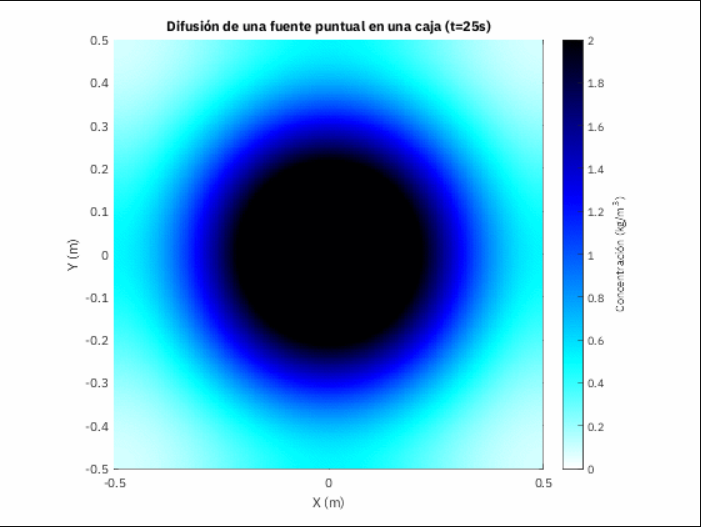
\includegraphics[width=.3\paperwidth]{E_IMAGENES/1_Capitulo2/25.png}\qquad
    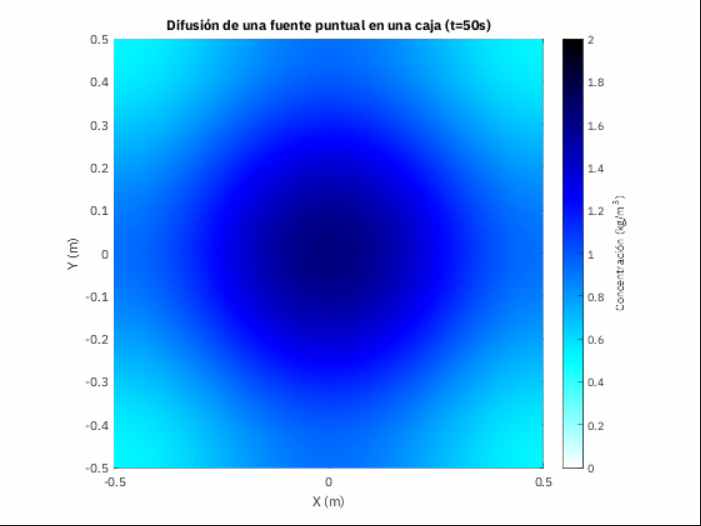
\includegraphics[width=.3\paperwidth]{E_IMAGENES/1_Capitulo2/50.png}
    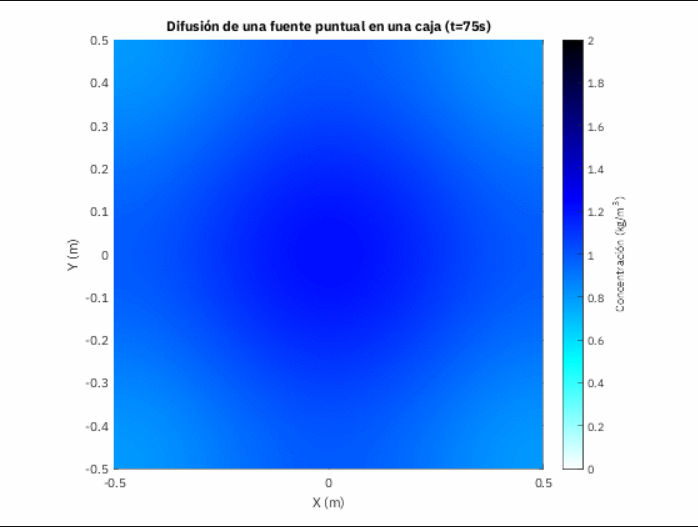
\includegraphics[width=.3\paperwidth]{E_IMAGENES/1_Capitulo2/75.png}\qquad
    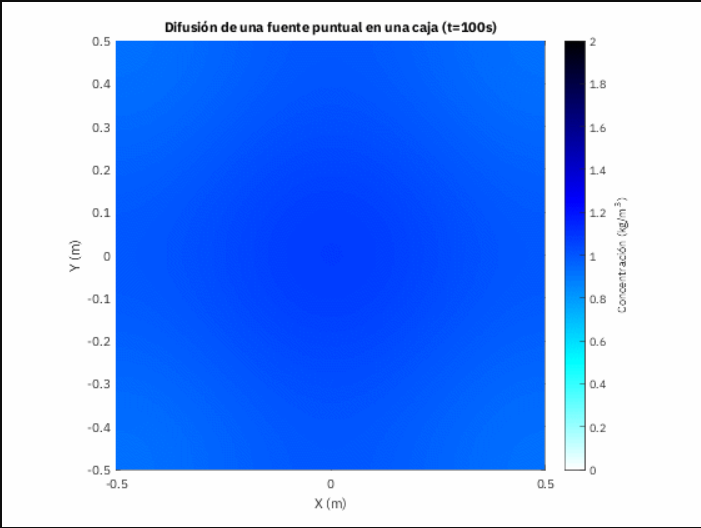
\includegraphics[width=.3\paperwidth]{E_IMAGENES/1_Capitulo2/100.png}
    \caption[corto]{Un tinte que se difunde en el agua en los tiempos
        $25$s, $50$s, $75$s y $100$s.
        En promedio, las partículas se mueven de regiones de mayor a menor densidad.}
\end{figure}

\begin{table}[ht!]
    \centering
    \begin{tabular}{ll}
        \textbf{Convección}                              &
        \textbf{Difusión}                                  \\
        Transporte de la magnitud por el flujo           &
        Efecto de las colisiones moleculares               \\
        \hline
        No existe en un fluido en reposo                 &
        Existe en un fluido en reposo                      \\
        \hline
        Comportamiento direccional                       &
        Comportamiento isotrópico                          \\
        \hline
        Derivadas espaciales de primer orden             &
        Derivadas espaciales de segundo orden              \\
        \hline
        No lineal, la velocidad del flujo depende de $U$ &
        Lineal, propiedades del fluido constantes
    \end{tabular}
    \caption[short]{Diferencias entre la convección y difusión.}
\end{table}

\begin{definition}[Concentración media]
    Sea $h>0$, $h\ll 1$.
    Definimos la \emph{concentración media}
    \begin{math}
        \averageconcentration
    \end{math}
    in a space-time cell
    \begin{math}
        \left[
            x-\frac{1}{2}h,
            +x\frac{1}{2}h
            \right]
        \times
        \left[
            0,T
            \right]
    \end{math}.

    \begin{equation*}
        \averageconcentration=
        \dfrac{1}{h}
        \int_{x-\frac{1}{2}h}^{x+\frac{1}{2}h}
        u
        \left(
        s,t
        \right)
        \dl s.
    \end{equation*}
\end{definition}

Sea
\begin{math}
    u\left(x,t\right)
\end{math}
la función concentración o densidad de alguna sustancia química.

\begin{definition}[Ecuación lineal de Advección-Difusión-Reacción]
    Para cualquier $x\in\Omega$ y $t\in\left[0,T\right]$,
    \begin{equation}\label{eq:advecion-difussion-reaction}
        \diffp{\phi}{t}\left(x,t\right)+
        u\left(x\right)\cdot
        \nabla\phi\left(x,t\right)=
        \nabla\cdot\left(a\left(x\right)\nabla\phi\left(x,t\right)\right)-
        c\left(x\right)\phi\left(x,t\right)
        +f\left(x,t\right)
    \end{equation}
\end{definition}

\begin{description}
    \item[Advección-Difusión]
        Si $u\equiv0$, entonces
        \begin{equation*}
            \diffp{\phi}{t}\left(x,t\right)=
            \nabla\cdot\left(a\left(x\right)\nabla\phi\left(x,t\right)\right)-
            c\left(x\right)\phi\left(x,t\right)
            +f\left(x,t\right)
        \end{equation*}

    \item[De difusión]
        Si $u\equiv0$, $c\equiv0$ y $f\equiv0$, entonces

        \begin{equation*}
            .
        \end{equation*}

    \item[De transporte lineal]

        \begin{equation*}
            .
        \end{equation*}
\end{description}

\begin{theorem}[Identidades integrales]
    Sea
    \begin{math}
        \Omega\subset
        \mathbb{R}^{d}
    \end{math}
    un dominio acotado con frontera suficientemente suave
    y
    \begin{math}
        n\colon
        \partial\Omega\to
        \mathbb{R}^{d}
    \end{math}
    normal unitario hacia afuera.
    Se cumplen
    \begin{description}
        \item[Integración por partes.]

            Si $u,v\in C^{1}\left(\overline{\Omega}\right)$, entonces
            \begin{equation*}
                \int_{\Omega}\diffp{u\left(x\right)}{x_{i}}
                v\left(x\right)\dl x=
                \int_{\partial\Omega}
                u\left(x\right)
                v\left(x\right)
                n\left(x\right)\cdot
                e_{i}
                \dl{S\left(x\right)}-
                \int_{\Omega}u\left(x\right)
                \diffp{v\left(x\right)}{x_{i}}
                \dl x.
            \end{equation*}

        \item[Primera identidad de Green.]
            Si $v\in C^{1}\left(\overline{\Omega}\right)$ y
            $w\in C^{2}\left(\overline{\Omega}\right)$, entonces
            \begin{equation*}
                \int_{\Omega}\nabla v\left(x\right)\cdot
                w\left(x\right)\dl x=
                -\int_{\Omega}
                v\left(x\right)
                \Delta w\left(x\right)
                \dl x+
                \int_{\partial\Omega}
                v\left(x\right)
                \diffp{w\left(x\right)}{n}
                \dl{S\left(x\right)},
            \end{equation*}
            donde
            \begin{math}
                \diffp{w\left(x\right)}{n}=
                n\left(x\right)\cdot
                \nabla w\left(x\right)
            \end{math}.

        \item[Segunda identidad de Green.]

            Si $v,w\in C^{2}\left(\overline{\Omega}\right)$, entonces
            \begin{equation*}
                \int_{\Omega}
                \left(
                v\left(x\right)
                \Delta w\left(x\right)-
                \Delta v\left(x\right)
                w\left(x\right)
                \right)
                \dl x=
                \int_{\partial\Omega}
                \left(
                v\left(x\right)
                \diffp{w}{n}\left(x\right)-
                \diffp{v}{n}\left(x\right)
                w\left(x\right)
                \right)
                \dl{S\left(x\right)}.
            \end{equation*}

        \item[]

            Si $v\in C^{1}\left(\overline{\Omega};\mathbb{R}^{d}\right)$ y
            $w\in C^{1}\left(\overline{\Omega}\right)$, entonces
            \begin{equation*}
                \int_{\Omega}\nabla\cdot v\left(x\right)
                w\left(x\right)
                \dl x=
                \int_{\partial\Omega}
                v\left(x\right)\cdot
                n\left(x\right)
                w\left(x\right)
                \dl{S\left(x\right)}-
                \int_{\Omega}
                v\left(x\right)\cdot
                \nabla w\left(x\right)
                \dl x.
            \end{equation*}
    \end{description}
\end{theorem}

La conservación de la masa conlleva a la ecuación de continuidad.

\subsection{Aproximaciones de diferencias finitas de las derivadas}

Si $u\colon\mathbb{R}^d\to\mathbb{R}$ es una función suficientemente
suave y
\begin{equation*}
    \forall i=1,\dotsc d:\quad
    \diffp{u\left(x\right)}{x_{i}}=
    \lim\limits_{h\to0}
    \dfrac{
        u\left(x+he_{i}\right)-
        u\left(x\right)}{h},
\end{equation*}

donde $e_{i}$ es el $i$-ésimo vector de la base canónica de
$\mathbb{R}^d$.

El método de las diferencias finitas surge al aproximar la derivada
de una función por una expresión de diferencias de valores de esta en
ciertos puntos discretos cercanos, y así, convertimos una ecuación
diferencial en un sistema finito de ecuaciones algebraicas que puede
ser resuelto en la computadora.
La elección de esta ``diferencia finita'' debería ser

\begin{description}
    \item[Consistente:]

        La aproximación sea tan precisa como sea posible y encontrar
        una aproximación de diferencia finita de las derivadas que
        sea consistente con el orden más alto posible.

    \item[Estable:]

        No solo con respecto a perturbaciones de los datos, sino
        en las versiones discretas de las mismas normas en las que la
        solución al problema continuo posee sus propias propiedades
        estabilidad.
\end{description}

% TODO: p. 103. [Hundsdorfer]
Una condición necesaria para la estabilidad es que el dominio de
dependencia de la ecuación diferencial parcial esté contenida en el
dominio de dependencia numérico, y en los problemas lineales es
conocido como

% TODO: p. 46 [Lax].
\begin{theorem}[Teorema de Equivalencia de Lax-Richtmyer]
    Un problema de valor inicial bien planteado y una aproximación de
    diferencia finita que satisface la condición de consistencia y
    estabilidad es una condición necesaria y suficiente para la
    convergencia.
\end{theorem}

\begin{figure}[ht!]
    \centering
    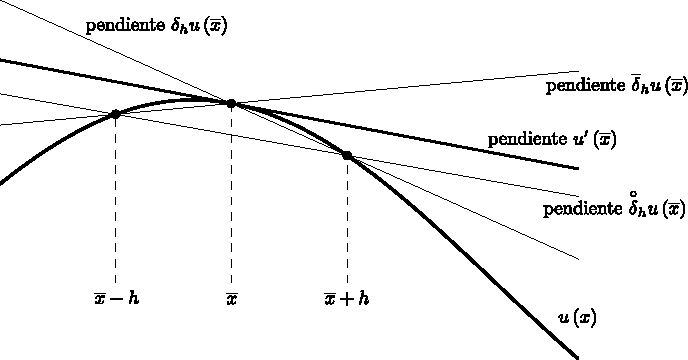
\includegraphics[width=.5\paperwidth]{E_IMAGENES/1_Capitulo2/finite_difference.pdf}
    \caption{
        Ilustración de los operadores de diferencias finitas usuales.
        Adaptado de~\citep{leveque_numerical_1992}.
    }
\end{figure}

Ahora, presentaremos algunas definiciones generales acerca de las
discretizaciones que nos permitirá estudiar la consistencia y
estabilidad de los esquemas venideros.

\subsection{Consistencia y Estabilidad de los Métodos de Diferencias Finitas}

Sean
\begin{math}
    \left(
    \mathbb{V},
    {\left\|\cdot\right\|}_{\mathbb{V}}
    \right)
\end{math},
\begin{math}
    \left(
    \mathbb{F},
    {\left\|\cdot\right\|}_{\mathbb{F}}
    \right)
\end{math}
y
\begin{math}
    \left(
    \mathbb{G},
    {\left\|\cdot\right\|}_{\mathbb{G}}
    \right)
\end{math}
tres espacios normados, donde el primero es de funciones definidas
sobre $\overline{\Omega}={\left[0,1\right]}^{d}$.
Encuentre un $u\in\mathbb{V}$ tal que
\begin{equation}\label{eq:boundary_value_problem}
    \begin{cases}
        Lu=f,     & \text{ en }\Omega,         \\
        \ell u=g, & \text{ en }\partial\Omega,
    \end{cases}
\end{equation}
donde $L$ y $\ell$ son operadores diferenciables.
El primero está asociado con la ecuación diferencial y el segundo con
las condiciones de frontera.
Las funciones $f\colon\Omega\to\mathbb{R}$ y
$g\colon\partial\Omega\to\mathbb{R}$
son elementos de $\mathbb{F}$ y $\mathbb{G}$, respectivamente.

Encuentre un $w\in\mathcal{V}\left(\overline{\Omega}_{h}\right)$ tal
que
\begin{equation}\label{eq:boundary_value_problem_finite}
    \begin{cases}
        L_{h}w=f_{h},    & \text{ en }\Omega^{I}_{h}, \\
        \ell_{h}w=g_{h}, & \text{ en }\Omega^{B}_{h},
    \end{cases}
\end{equation}
donde $L_{h}$ y $\ell_{h}$ son operadores de diferencias finitas,
\begin{math}
    \Omega^{I}_{h}
\end{math}
y
\begin{math}
    \Omega^{B}_{h}
\end{math}
son los puntos malla interiores y frontera, respectivamente.

Sea
\begin{math}
    \left\{
    \left(
    \mathcal{V}\left(\overline{\Omega}_{h}\right),
    \left\|\cdot\right\|_{h}
    \right)
    \right\}_{h>0}
\end{math}
la aproximación con respecto a
\begin{math}
    \left(
    \mathbb{V},
    {\left\|\cdot\right\|}_{\mathbb{V}}
    \right)
\end{math}.

\begin{definition}[Estabilidad]
    Decimos que el MDF~\eqref{eq:boundary_value_problem_finite} es
    estable sii existen $h_{0}>0$ y $C>0$ tales que
    \begin{math}
        \forall h\in\left(0,h_{0}\right]
    \end{math},
    el problema~\eqref{eq:boundary_value_problem}
    tiene una única solución para cualquier
    \begin{math}
        \left(
        f_{h},g_{h}
        \right)\in
        \mathcal{V}\left(
        \Omega^{I}_{h}
        \right)\times
        \left(
        \mathcal{V}\left(
            \Omega^{B}_{h}
            \right)
        \right)
    \end{math}
    y
    \begin{equation*}
        \left\|w\right\|_{h}\leq
        C\left(
        \left\|f_{h}\right\|_{\mathcal{V}\left(
            \Omega^{I}_{h}
            \right)}+
        \left\|g_{h}\right\|_{\mathcal{V}\left(
            \Omega^{B}_{h}
            \right)}
        \right)
    \end{equation*}
    donde
    \begin{math}
        {\left\|\cdot\right\|}_{\mathcal{V}\left(
            \Omega^{I}_{h}
            \right)}
    \end{math}
    y
    \begin{math}
        {\left\|\cdot\right\|}_{\mathcal{V}\left(
            \Omega^{B}_{h}
            \right)}
    \end{math}
    son normas que tienen la propiedad de aproximación con respecto a
    \begin{math}
        \left(
        \mathbb{F},
        {\left\|\cdot\right\|}_{\mathbb{F}}
        \right)
    \end{math}
    y
    \begin{math}
        \left(
        \mathbb{G},
        {\left\|\cdot\right\|}_{\mathbb{G}}
        \right)
    \end{math},
    respectivamente.
\end{definition}

Sea
\begin{math}
    \left\{
    \left(
    \mathcal{V}\left(\overline{\Omega}_{h}\right),
    \left\|\cdot\right\|_{h}
    \right)
    \right\}_{h>0}
\end{math}
la aproximación con respecto a
\begin{math}
    \left(
    \mathbb{V},
    {\left\|\cdot\right\|}_{\mathbb{V}}
    \right)
\end{math}.

\begin{definition}[Operador de consistencia]
    Sea
    \begin{math}
        L\colon\mathbb{V}\to\mathbb{V}
    \end{math}
    un operador lineal, no necesariamente acotado y
    \begin{math}
        L_{h}\colon
        \mathcal{V}\left(\mathbb{Z}^{d}_{h}\right)\to
        \mathcal{V}\left(\mathbb{Z}^{d}_{h}\right)
    \end{math}
    un operador de diferencia finita.
    Definimos el error de consistencia en $v\in\mathbb{V}$
    \begin{equation*}
        \forall x\in\mathbb{Z}^{d}_{h}:
        \mathcal{E}_{h}\left[L,v\right]\left(x\right)=
        \left(L_{h}\pi_{h}v-\pi_{h}\left(Lv\right)\right)
        \left(x\right).
    \end{equation*}
    Decimos que el operador de diferencia finita $L_{h}$ es
    consistente al menos de orden $p\in\mathbb{N}$ con $L$ sii
    existen $k\in\mathbb{N}$, $h_{1}>0$ tales que para cualquier
    \begin{math}
        h\in\left(0,h_{1}\right]
    \end{math}
    y
    \begin{math}
        v\in C^{k}\left(\mathbb{R}^{d}\right)
    \end{math}
    \begin{equation*}
        {\left\|\varepsilon_{h}\left[L,v\right]\right\|}_{h}\leq
        C h^{p}.
    \end{equation*}
\end{definition}

\begin{definition}[Consistencia]
    Definimos el error de consistencia
    de~\eqref{eq:boundary_value_problem_finite}
    \begin{equation*}
        \mathcal{E}_{h}
        \left[u\right]
        \left(x\right)=
        \begin{cases}
            \left(L_{h}\pi_{h}u-f_{h}\right)\left(x\right) \\
            \left(\ell_{h}\pi_{h}u-g_{h}\right)\left(x\right)
        \end{cases}
    \end{equation*}
    donde $u\in\mathbb{V}$
    resuelve~\eqref{eq:boundary_value_problem}.
    Decimos que el MDF~\eqref{eq:boundary_value_problem_finite} es
    consistente al menos de orden $p\in\mathbb{N}$
    con~\eqref{eq:boundary_value_problem} sii existen
    $k\in\mathbb{N}$ tal que si
    \begin{math}
        u\in C^{k}\left(\overline{Omega}_{h}\right)
    \end{math},
    entonces existen $h_{1}>0$ y $C>0$ tales que
    \begin{math}
        \forall h\in\left(0,h_{1}\right]:
        {
        \left\|\mathcal{\varepsilon}_{h}\left[u\right]\right\|
        }_{\mathcal{V}\left(\Omega^{I}_{h}\right)}+
        {
        \left\|\mathcal{\varepsilon}_{h}\left[u\right]\right\|
        }_{\mathcal{V}\left(\Omega^{B}_{h}\right)}\leq
        C h^{p}
    \end{math}.
\end{definition}

\begin{proposition}[Consistencia]
    Sea $d=1$. Tenemos
    \begin{enumerate}
        \item

              El operador de diferencia hacia adelante es consistente
              sobre
              \begin{math}
                  C_{b}\left(\mathbb{R}\right)
              \end{math}
              hasta exactamente orden uno con.

        \item

              El operador de diferencia hacia atrás es consistente.

        \item

              El operador de diferencia centrada es consistente.
    \end{enumerate}
\end{proposition}

\begin{definition}[Malla uniforme]
    Sean $N\in\mathbb{N}$.
    El tamaño de la malla es
    \begin{math}
        h=
        \dfrac{1}{N+1}
    \end{math}
    y la malla uniforme es
    \begin{equation*}
        \mathbb{Z}^{d}_{h}\coloneqq
        \left\{
        hz\in\mathbb{R}^{d}\mid
        z\in\mathbb{Z}^{d}
        \right\}.
    \end{equation*}
\end{definition}

\begin{definition}[Conjunto de funciones malla]
    \begin{math}
        \emptyset\neq\mathcal{G}_{h}\subset
        \mathbb{Z}^{d}_{h}
    \end{math}
    es un dominio malla.
    Los puntos $x\in\mathcal{G}_{h}$ son los nodos o puntos de la
    malla.
    Se define el conjunto de funciones malla sobre $\mathcal{G}_{h}$
    como
    \begin{equation*}
        \mathcal{V}
        \left(\mathcal{G}_{h}\right)\coloneqq
        \left\{
        v\mid v\colon\mathcal{G}_{h}\to\mathbb{R}
        \right\}.
    \end{equation*}
    Además,
    \begin{math}
        \forall v\in\mathcal{V}\left(\mathcal{G}_{h}\right):
        \forall hi\in\mathcal{G}_{h}:
        v_{i}=
        v\left(hi\right)
    \end{math}.
\end{definition}

\begin{definition}[Espacio $\mathcal{V}_{0}\left(\overline{\Omega}_{h}\right)$]
    Sean
    \begin{math}
        \Omega=
        {\left(0,1\right)}^{d}
    \end{math},
    \begin{math}
        N\in\mathbb{N}
    \end{math},
    \begin{math}
        h=
        \dfrac{1}{\left(N+1\right)}
    \end{math}
    y
    \begin{math}
        \overline{\Omega}_{h}=
        \overline{\Omega}\cap
        \mathbb{Z}^{d}_{h}
    \end{math}.

    \begin{equation*}
        \mathcal{V}_{0}\left(\overline{\Omega}_{h}\right)\coloneqq
        \left\{
        v\in\mathcal{V}\left(\overline{\Omega}_{h}\right)
        \right\}
    \end{equation*}
\end{definition}

\begin{definition}[Operador diferencia finita]
    La aplicación
    \begin{equation*}
        \mathcal{F}_{h}\colon
        \mathcal{V}\left(\mathbb{Z}^{d}_{h}\right)\to
        \mathcal{V}\left(\mathbb{Z}^{d}_{h}\right)
    \end{equation*}
    es llamada \emph{operador de diferencia finita} sii
    \begin{equation*}
        \forall x\in\mathbb{Z}^{d}_{h}:
        \left(\mathcal{F}_{h}u\right)\left(x\right)=
        \sum_{e\in S}
        a_{e}\left(x,h\right)
        \left(\mathcal{S}_{e}v\right)
        \left(x\right),
    \end{equation*}
    donde $S\subset\mathbb{Z}^{d}_{h}$ es finito y $0\in S$.
\end{definition}

Sea un dominio espacio-temporal contenido en $\mathbb{R}^{d+1}$.

\begin{definition}[Dominio malla espacio-temporales]
    Sean
    \begin{math}
        \Omega=
        {\left(0,1\right)}^{d}
    \end{math},
    $T>0$, $K,N\in\mathbb{N}$.
    \begin{equation*}
        \overline{\mathcal{C}}^{\tau}_{h}\coloneqq
        \overline{\Omega}_{h}
        \times
        {\left[0,T\right]}_{\tau}=
        \left\{
        \left(x,t_{k}\right)\mid
        x\in\overline{\Omega}_{h},
        t_{k}=k\tau,
        k=0,\dotsc, K
        \right\}.
    \end{equation*}
\end{definition}

\begin{definition}[Interior discreto de $\overline{\mathcal{C}}^{\tau}_{h}$]
    \begin{equation*}
        \overline{\mathcal{C}}^{\tau}_{h}\coloneqq
        \Omega_{h}\times
        {\left(0,T\right)}_{\tau}.
    \end{equation*}
\end{definition}

\begin{definition}[Frontera lateral discreta]
    \begin{equation*}
        \partial_{L}
        \mathcal{C}^{\tau}_{h}\coloneqq
        \partial\Omega_{h}\times
        {\left[0,T\right]}_{\tau}.
    \end{equation*}
\end{definition}

\begin{definition}[Frontera parabólica discreta]
    \begin{equation*}
        \partial_{p}
        \mathcal{C}^{\tau}_{h}\coloneqq
        \overline{\Omega}_{h}\times
        \left\{0\right\}\cup
        \partial_{L}
        \mathcal{C}^{\tau}_{h}.
    \end{equation*}
\end{definition}

\begin{definition}[Espacio de funciones malla espacio-temporales]
    Sea $\mathcal{C}^{\tau}_{h}$ un dominio malla espacio-temporales.
    El espacio de funciones
    \begin{align*}
        \mathcal{V}
        \left(
        \overline{\mathcal{C}}^{\tau}_{h}
        \right) & =
        \left\{
        v\mid
        \overline{\mathcal{C}}^{\tau}_{h}\to\mathbb{R}
        \right\}.   \\
        \mathcal{V}
        \left(
        \mathcal{C}^{\tau}_{h}
        \right) & =
        \left\{
        v\mid
        \mathcal{C}^{\tau}_{h}\to\mathbb{R}
        \right\}.   \\
        \mathcal{V}
        \left(
        \partial_{L}\mathcal{C}^{\tau}_{h}
        \right) & =
        \left\{
        v\mid
        \partial_{L}\mathcal{C}^{\tau}_{h}\to\mathbb{R}
        \right\}.   \\
        \mathcal{V}_{0}
        \left(
        \overline{\mathcal{C}}^{\tau}_{h}
        \right) & =
        \left\{
        v\in
        \mathcal{V}\left(\overline{\mathcal{C}}^{\tau}_{h}\right)\mid
        v\left(x,t\right)=0,
        \forall\left(x,t\right)\in\partial_{L}\mathcal{C}^{\tau}_{h}
        \right\}.   \\
        \mathcal{V}
        \left(
        \overline{\Omega}_{h}
        \right) & =
        \left\{
        v^{k}\mid
        v\in
        \mathcal{V}
        \left(
        \overline{\mathcal{C}}^{\tau}_{h}
        \right),
        v^{k}\left(x\right)=
        v\left(x,k\tau\right)
        \forall x\in\overline{\Omega}_{h}
        \right\}
    \end{align*}
\end{definition}

Los espacios de funciones malla espacio-temporales pueden
identificarse como un espacio de funciones de valor función malla
espacial, o sea

\begin{align*}
    \mathcal{V}
    \left(
    \overline{\mathcal{C}}^{\tau}_{h}
    \right) & =
    \mathcal{V}
    \left(
    \left[0,T\right]_{\tau};
    \mathcal{V}
    \left(\overline{\Omega}_{h}\right)
    \right)=
    {
    \left(
    \mathcal{V}\left(\overline{\Omega}_{h}\right)
    \right)
    }^{K+1}.    \\
    \mathcal{V}_{0}
    \left(
    \overline{\mathcal{C}}^{\tau}_{h}
    \right) & =
    \mathcal{V}
    \left(
    \left[0,T\right]_{\tau};
    \mathcal{V}_{0}\left(\overline{\Omega}_{h}\right)
    \right).
\end{align*}

\begin{definition}
    Sean
    \begin{math}
        d\in\left\{1,2\right\}
    \end{math},
    \begin{math}
        p\in
        \left[1,\infty\right)
    \end{math}
    y
    \begin{math}
        q\in\left[1,\infty\right)
    \end{math}.

    \begin{align*}
        {\left\|v\right\|}_{
            L^{q}_{\tau}\left(L^{p}_{h}\right)
        }
         & =
        {\left(
        \tau\sum_{k=1}^{K}
        \left\|v^{k}\right\|^{q}_{L^{p}_{h}}
        \right)}^{\frac{1}{q}}. \\
        {\left\|v\right\|}_{L^{\infty}_{\tau}\left(L^{p}_{h}\right)}
         & =
        \max^{K}_{k=0}
        {\left\|v^{k}\right\|}_{L^{p}_{h}}.
    \end{align*}
\end{definition}

\begin{definition}[Número de Courant]
    Sea $\overline{\mathcal{C}}^{\tau}_{h}$ una malla
    espacio-temporal.
    El número de Courant parabólico es
    \begin{equation*}
        \mu=
        \dfrac{\tau}{h^{2}}.
    \end{equation*}
\end{definition}

\begin{definition}[Estabilidad condicional]
    Decimos que un método de diferencia finita es
    \emph{condicionalmente estable} sii este es estable.
\end{definition}

\begin{equation*}
    U^{n+1}_{j}=
    U^{n}_{j}-
    \dfrac{\lambda}{2}
    \left(U^{n}_{j+1}-U^{n}_{j}\right)+
    \dfrac{\lambda^{2}}{2}
    \left(
    U^{n}_{j+1}-
    2U^{n}_{j}+
    U^{n}_{j-1}
    \right)
\end{equation*}
	\input{2_CAPITULO1/Secciones/2_Descripción del problema.tex}
	\section{OBJETIVOS DEL ESTUDIO}
\subsection{Objetivo General}

Comparar algunos resultados de convergencia de ciertos problemas
test de advección-difusión y explicar la precisión y estabilidad del método.

\subsection{Objetivos Específicos}
\begin{itemize}
	\item Objetivo específico 1.

	\item Objetivo específico 2.
\end{itemize}

\subsection{Variables de investigación}

\begin{itemize}
	\item Independientes

	      \begin{itemize}
		      \item Los esquemas numéricos: Upwind, Lax-Wendroff.
		      \item Condiciones iniciales y/o de contorno de la ecuación de advección-difusión.
	      \end{itemize}

	\item Dependientes
	      \begin{itemize}
		      \item Error (diferencia entre la solución aproximada y la exacta).
		      \item Estabilidad del método.
	      \end{itemize}
\end{itemize}	
	% \input{2_CAPITULO1/Secciones/4_Hipótesis.tex}
	% \input{2_CAPITULO1/Secciones/5_Metodología.tex}
% % FUNDAMENTO TEÓRICO Y CONCEPTUAL
% \chapter{FUNDAMENTO TEÓRICO Y CONCEPTUAL}
\markboth{CAPÍTULO \thechapter: MARCO TEÓRICO Y CONCEPTUAL}{}

% \lipsum[3]

\section{Esquemas numéricos}
% \subsection{Aisladores Sísmicos}
% Son dispositivos que desacoplan la estructura y su contenido de los efectos de un sismo. Este desacople se alcanza incrementando la flexibilidad del sistema y proporcionándole un amortiguamiento adecuado \shortcites{Skinner1993}\citep{Skinner1993}.

% Existen diversos tipos de aisladores sísmicos, siendo los más usados en la actualidad los aisladores elastoméricos y los aisladores friccionantes.

% \subsubsection{Aisladores Elastoméricos}
% \begin{itemize}

% 	\item Aisladores de elastómero natural o de bajo amortiguamiento

% 	      Los dispositivos NRB (\textit{Natural Rubber Bearing}) consisten en capas alternadas de caucho y acero unidas mediante un proceso de vulcanización. Se caracterizan por su bajo nivel de amortiguamiento (alrededor de 2-3\%), poseen una curva fuerza deformación casi lineal y una fuerza restitutiva estable \citep{Kelly1999}.

% \end{itemize}

% \subsubsection{Aisladores Friccionantes}
% \begin{itemize}

% 	\item Aisladores de péndulo de fricción simple

% 	      Los dispositivos FPS (\textit{Frictional Pendulum System}) constan de un deslizador articulado que se mueve sobre una superficie de fricción esférica. La superficie de contacto está revestida de un material compuesto autolubricante. Cuando el deslizador se mueve sobre la superficie esférica, la masa soportada se levantará y el movimiento proporcionará la fuerza restitutiva del sistema. El radio de curvatura de la superficie cóncava dominará la rigidez y el periodo del sistema \citep{Wu2001}.

% \end{itemize}


% \begin{figure}[!h]
% 	\centering
% 	\begin{subfigure}[b]{0.45\textwidth}
% 		\centering
% 		% include first image
% 		\includegraphics[scale=1]{E_IMAGENES/1_Capitulo2/Cap2_Imagen1a.pdf}
% 		\caption{\centering\footnotesize Aislador eslastomérico LRB. Adaptado de \citet{Bridgestone2015}}
% 		\label{Cap2_Figura1a}
% 	\end{subfigure}
% 	\hfill
% 	\begin{subfigure}[b]{0.45\textwidth}
% 		\centering
% 		% include second image
% 		\includegraphics[scale=1]{E_IMAGENES/1_Capitulo2/Cap2_Imagen1b.pdf}
% 		\caption{\centering\footnotesize Aislador friccionante TFPB. Adaptado de \citet{Fenz2008}}
% 		\label{Cap2_Figura1b}
% 	\end{subfigure}
% 	\caption[Dispositivos de aislamiento sísmico]{\centering\footnotesize Dispositivos de aislamiento sísmico}
% 	\label{Cap2_Figura1}
% \end{figure}

% \subsection{Disipadores de Fluido Viscoso}
% Son dispositivos que incrementan el amortiguamiento de la estructura sin incrementar la rigidez y cuyo funcionamiento depende fundamentalmente de la velocidad relativa de sus extremos. Los DFV están compuestos por un pistón de acero inoxidable, con cabezal de bronce y un acumulador, que se encuentran alojados dentro en un cilindro metálico lleno con un fluido de alta viscosidad. La cabeza del pistón tiene orificios que están diseñados con una serie de formas especiales para alterar las características de flujo con la velocidad del fluido, disipando de esta manera energía en forma de calor. La construcción mecánica y las propiedades del orificio se pueden variar para obtener las propiedades amortiguadoras deseadas \citep{Constantinou1993}.

% \begin{figure}[!h]
% 	\centering
% 	\includegraphics[scale=1]{E_IMAGENES/1_Capitulo2/Cap2_Imagen2.pdf}
% 	\caption[Disipador de fluido viscoso]{\centering\footnotesize Disipador de fluido viscoso.  Adaptado de \shortcites{Taylor2019}\citet{Taylor2019}}
% 	\label{Cap2_Figura2}
% \end{figure}

\subsection{El método Upwind}

\subsection{El método Lax-Wendroff}


% \section{SEGUNDO TEMA}

En esta sección se revisan modelos matemáticos capaces de describir de forma analítica una amplia gama de comportamientos inelásticos complejos presentes en muchos sistemas y materiales.

\subsection{Modelo Histerético de Bouc-Wen} \label{subsection:MHBW}

Es un modelo que se usa para predecir el comportamiento dinámico no lineal de aisladores sísmicos, así como de disipadores histeréticos. El modelo de Bouc-Wen necesita cuatro parámetros de entrada, los cuales son: la rigidez elástica, la rigidez postfluencia, la fuerza característica y un parámetro adimensional que controla la forma del lazo histerético.

De acuerdo con \citet{Charalampakis2010} la fuerza en el tiempo \textit{t} del modelo histerético de Bouc-Wen se evalúa en función del desplazamiento de la siguiente manera:
\begin{gather}
	F(t)=\alpha \frac{F_{y}}{D_{y}}u(t)+(1-\alpha)F_{y}z(t)				\label{BoucWen1} \\
	\begin{aligned}
		\dot{z}(t)=\left[1-\left|z(t)\right |^{\eta}sgn(\dot{u}(t)z(t))\right]\frac{\dot{u}(t)}{D_{y}} & , & \hspace{1em} & z(0)=0 \\
	\end{aligned}		\label{BoucWen2}
\end{gather}

\begin{figure}[!h]
	\centering
	\includegraphics[scale=1]{E_IMAGENES/1_Capitulo2/Cap2_Imagen6.pdf}
	%\vspace{-3 mm}
	\caption[Modelo histerético de Bouc-Wen]{\centering\footnotesize Modelo histerético de Bouc-Wen. Adaptado de \citet{Charalampakis2010}}
	\label{Cap2_Figura6}
\end{figure}

En la \autoref{Cap2_Figura6} y en las ecuaciones \ref{BoucWen1} y \ref{BoucWen2} se muestran los parámetros necesarios para definir un ciclo histerético con comportamiento de Bouc-Wen.

Donde:

%Inicar tabla explicando cada Parámetro
\begin{tabular}{L{0.5 cm}p{0.025 cm}p{11.5 cm}}
	$K_{e}$  & : & Rigidez elástica                                                  \\
	$K_{p}$  & : & Rigidez postfluencia                                              \\
	$Q$      & : & Fuerza característica                                             \\
	$D_{y}$  & : & Desplazamiento de fluencia                                        \\
	$F_{y}$  & : & Fuerza de fluencia                                                \\
	$\alpha$ & : & Razón entre la rigidez postfluencia y la rigidez elástica         \\
	$\eta$   & : & Parámetro adimensional que controla la forma del lazo histerético \\
\end{tabular}\\





% \section{TERCER TEMA}
 
	\subsection{Modelo de Masas Concentradas}
	
Es un modelo físico discreto conformado por una serie de masas interconectadas por resortes sin peso (sistema de acoplamiento cercano). Este modelo puede describir adecuadamente el comportamiento de edificaciones con un sistemas estructural basado en pórticos con vigas muy rígidas y donde las deformaciones axiales de las columnas se desprecian.

		\subsubsection{Matrices de Masa y Rigidez}

Para un modelo discreto de masas concentradas de $n$ GDL, la matriz de masas $\mathbfit{M}$ es diagonal, con la masa $i_{\acute{e}sima}$, $m_{i}$, como el elemento diagonal $i_{\acute{e}simo}$.

\begin{equation}\label{Eq18}
M=\begin{bmatrix}
m_{1} & 0 & 0 & \cdots & 0 & 0 \\ 
0 & m_{2} & 0 & \cdots & 0 & 0\\ 
0 & 0 & m_{3} & \cdots & 0 & 0\\ 
\vdots & \vdots & \vdots &\ddots  &\vdots  &\vdots \\ 
0 & 0 & 0 & \cdots & m_{n-1}& 0\\ 
0 & 0 & 0 & \cdots & 0 & m_{n}
\end{bmatrix}_{n\times n}
\end{equation}



		\subsubsection{Matriz de Amortiguamiento}

Usando el amortiguamiento de Rayleigh se puede construir una matriz de amortiguamiento que sea consisten con los datos experimentales \citep{Chopra2016}. Tal como se aprecia en la ecuación \ref{Eq21}, Rayleigh propone que la matriz de amortiguamiento sea una combinación lineal de la matriz de masa y la matriz de rigidez.
\begin{equation}\label{Eq21}
\mathbfit{C}=a_{0}\mathbfit{M}+a_{1}\mathbfit{K}
\end{equation}








% \section{CUARTO TEMA}

De acuerdo con la ASCE 7-16 y la norma E.031 cuando se realice un análisis tiempo historia para diseñar edificaciones que incorporen algún sistema de control pasivo se debe usar un mínimo de siete registros sísmico, los cuales deben estar escalados correctamente. Dado que el objetivo de la presente tesis no es realizar un diseño detallado sino más bien conocer la eficiencia de cada sistema de control pasivo en la reducción de la respuesta sísmica, se usaron solo tres registros.

\subsection{Registros Sísmicos Ajustados}

A continuación se presentan los registros sísmicos usados en la presente tesis.

\begin{figure}[h!]
	\centering
	\includegraphics[scale=1]{E_IMAGENES/1_Capitulo2/Cap2_PiscoSc.pdf}
	\vspace{-8 mm}
	\caption[Acelerogramas espectrocompatibles - Pisco 2007]{\centering\footnotesize Acelerogramas espectrocompatibles - Pisco 2007.}
	\label{Cap2_Figura15}
\end{figure}

% % CAPÍTULO 3
% \chapter{NOMBRE DEL CAPÍTULO 3}
\markboth{CAPÍTULO \thechapter: NOMBRE DEL CAPÍTULO 3}{}

\lipsum [6]

	\input{2_CAPITULO3/Secciones/1_Primera Sección.tex}
	
	\input{2_CAPITULO3/Secciones/2_Segunda Sección.tex}
	
	\input{2_CAPITULO3/Secciones/3_Tercera Sección.tex}
	
	\input{2_CAPITULO3/Secciones/4_Cuarta Sección.tex}




		


% % CAPÍTULO 4
% \chapter[NOMBRE DEL CAPÍTULO 4]{NOMBRE DEL CAPÍTULO 4}
\markboth{CAPÍTULO \thechapter: NOMBRE DEL CAPÍTULO 4}{}

% \lipsum[1]

% \input{2_CAPITULO4/Secciones/1_Primera Sección.tex}
% \input{2_CAPITULO4/Secciones/2_Segunda Sección.tex}


% %Parte FINAL DE LA TESIS
% \backmatter

% % CONCLUSIONES
% \cleardoublepage\phantomsection\addcontentsline{toc}{chapter}{\bf CONCLUSIONES}
\chapter*{\centerline {CONCLUSIONES}}
\markboth{CONCLUSIONES}{}
%--
\begin{enumerate}

	\item Nam dui ligula, fringilla a, euismod sodales, sollicitudin vel, wisi.  Morbiauctor lorem non justo. Nam lacus libero, pretium at, lobortis vitae, ultricies et,tellus. Donec aliquet, tortor sed accumsan bibendum, erat ligula aliquet magna,vitae ornare odio metus a mi.
\end{enumerate}

% % RECOMENDACIONES	
% \cleardoublepage\phantomsection\addcontentsline{toc}{chapter}{\bf RECOMENDACIONES}
\chapter*{\centerline {RECOMENDACIONES}}
\markboth{RECOMENDACIONES}{}
%
\begin{enumerate}
	\item Nam dui ligula, fringilla a, euismod sodales, sollicitudin vel, wisi.  Morbiauctor lorem non justo. Nam lacus libero, pretium at, lobortis vitae, ultricies et,tellus. Donec aliquet, tortor sed accumsan bibendum, erat ligula aliquet magna,vitae ornare odio metus a mi.
\end{enumerate}

% REFERENCIAS BIBLIOGRÁFICAS
\cleardoublepage\phantomsection\addcontentsline{toc}{chapter}{\bf Referencias Bibliográficas}
\begingroup
\titleformat*{\chapter}{\normalfont\bfseries\normalsize\centering}
\bibliography{3_3_BIBLIOGRAFIA/library}
\nocite{*}
\endgroup
% https://www.clawpack.org/riemann_book/html/riemann_bib.html#godunov1959difference

% ANEXOS
% \cleardoublepage\phantomsection\addcontentsline{toc}{chapter}{\bf ANEXOS}
\chapter*{\centerline {ANEXOS}}
\markboth{ANEXOS}{}
%---

% Definir númeración y citación para Listing

\renewcommand{\lstlistingname}{ \footnotesize Código A \hspace{-1.75mm}}% Cambiar el nombre a Algoritmo
\renewcommand*{\thelstlisting}{.\arabic{lstlisting}}
\def\lstlistingautorefname{Código A\hspace{-0.75mm}}

% Redefinir númeración y citación para Figuras
\renewcommand\thefigure{.\arabic{figure}}
\setcounter{figure}{0}
\renewcommand\figurename{\footnotesize FIGURA B \hspace{-1.6mm}}
\def\figureautorefname{Figura B \hspace{-2mm}}


\section*{ANEXO A: CÓDIGOS EN PYTHON}
\phantomsection
\addcontentsline{toc}{section}{ANEXO A: CÓDIGOS EN PYTHON}
A continuación se presentan los códigos desarrollados en \textit{Python}. En este sentido, el \autoref{Algoritmo1} muestra el algoritmo usado para edificaciones con aislamiento de base con comportamiento bilineal. El \autoref{Algoritmo2} muestra las funciones usadas por los algoritmos anteriormente mencionados.

\vspace*{2mm}

\subsection*{Respuesta Sísmica de una Edificación con AS}
%\phantomsubsection
\addcontentsline{toc}{subsection}{Respuesta Sísmica de una Edificación con AS}

\begin{MyFont}
\begin{adjustwidth}{4.8mm}{}
\begin{lstlisting}[language=Python, caption= {\footnotesize Edificación con aislamiento sísmico bilineal}, mathescape=true,label={Algoritmo1}]
# REPUESTA SÍSMICA DE UNA EDIFICACIÓN DE n NIVELES CON AS
import Funciones_KS as fun
import numpy as np
from scipy  import linalg as LA
import copy

# PROPIEDADES DINÁMICAS
# Parámetros dinámicos de la Superestructura
n=3                 # N° de Pisos
gdl=n+1             # GDL = N° de Pisos+1
Tnf=0.3             # Periodo base fija, [s]
$\xi$=5           			 # Amortiguamiento, [%]
$\lambda$=(gdl-1)/gdl 			 # Relación de masas

# Parámetros dinámicos de la interfaz de aislamiento
r=0.1               # Razón de rigideces Kp/Ke
Q=105          		  # Fuerza característica normalizada, [cm/s^2]
K2=30         		  # Rigidez postfluencia normalizada, [1/s^2]

# LECTURA DEL REGISTRO SÍSMICO
ug=np.genfromtxt("./Sismo_Lima66NS.txt")  #[cm/s^2]
$\Delta$t=0.002; N=len(ug)
t=[i*$\Delta$t for i in range(N)]

\end{lstlisting}
\end{adjustwidth}
\end{MyFont}

\subsection*{Funciones}
%\phantomsubsection
\addcontentsline{toc}{subsection}{Funciones}

\begin{MyFont}
\begin{adjustwidth}{4.8mm}{}
\begin{lstlisting}[language=Python, caption={\footnotesize Funciones-KS}, mathescape=true,label={Algoritmo2}]
import numpy as np
from scipy  import linalg as LA
import copy

# FUNCIÓN EIGEN
def eigen(Tsf=1,n=5):
    Z=np.identity(n); ke=(4*n/Tsf)**2; k=np.zeros(n)
    for i in range(n):
        if i==0:
            k[i]=2*ke
        else:
            k[i]=ke
    K=tridiag(k,n); M=np.identity(n)
    vp,$\varphi$p=LA.eigh(K,M); $\varphi$p=$\varphi$p.T; FP=[]; MP=[] 
    for i in range(n):
        FP.append(sum($\varphi$p[i].T@M))
    for i in range(n):
        MP.append((sum($\varphi$p[i].T@M))**2)
    T=2*np.pi/(vp)**0.5; MMP=MP/sum(MP)
    return T,$\varphi$p,FP,MMP

\end{lstlisting}
\end{adjustwidth}
\end{MyFont}


\newpage

\section*{ANEXO B: HISTÉRESIS DE LOS DISPOSITIVOS DE CONTROL}
\phantomsection
\addcontentsline{toc}{section}{ANEXO B: HISTÉRESIS DE LOS DISPOSITIVOS DE CONTROL}

\lipsum[10]

\subsection*{Edificio Principal del Aeropuerto Jorge Chavez}
%\phantomsubsection
\addcontentsline{toc}{subsection}{Edificio Principal del Aeropuerto Jorge Chavez}

La \autoref{Anexo_1} muestra las histéresis de uno de los dos los DFV instalados en el eje 5-5 del primer nivel del edificio pincipal del aeropuerto Jorge Chavez. Asimismo, la \autoref{Anexo_2} presenta la histéresis de uno de los tres DH-SLB colocado en el eje 5-5 del primer nivel de la misma edificación.


\begin{figure}[!h]
	\centering
	\includegraphics[scale=1]{E_IMAGENES/Anexos/Anexo_1.pdf}
	\vspace{-8 mm}
	\caption[]{\centering\footnotesize Histéresis del DFV del edificio del aeropuerto Jorge Chavez.}
	\label{Anexo_1}
\end{figure}


\begin{figure}[!h]
	\centering
	\includegraphics[scale=1]{E_IMAGENES/Anexos/Anexo_2.pdf}
	\vspace{-8 mm}
	\caption[]{\centering\footnotesize Histéresis del DH-SLB del edificio del aeropuerto Jorge Chavez.}
	\label{Anexo_2}
\end{figure}



\chapter*{Anexos}

% Cambiar nombre, crear ÍNDICE DE FIGURAS Y TABLAS
\renewcommand\listfigurename{\centering Lista de Figuras}
\renewcommand\listtablename{\centering Lista de Tabla}

% \cleardoublepage\phantomsection\addcontentsline{toc}{chapter}{\listtablename}
% {\normalsize\listoftables}
% \cleardoublepage\phantomsection\addcontentsline{toc}{chapter}{\listfigurename}
% {\normalsize\listoffigures}

\cleardoublepage\phantomsection\addcontentsline{toc}{chapter}{LISTA DE SÍMBOLOS Y SIGLAS}
\chapter*{\centerline {LISTA DE SÍMBOLOS Y SIGLAS}}
\markboth{LISTA DE SÍMBOLOS Y SIGLAS}{}

\section*{\textbf{\underline{SÍMBOLOS}}}

\begin{tabular}{L{1.5 cm}p{12.5 cm}}
    $\delta_{h}$                            &
    Operador de diferencia hacia adelante.                                                       \\
    $\overline{\delta}_{h}$                 &
    Operador de diferencia hacia atrás.                                                          \\
    ${\overset{\circ}{\delta}}_{h}$         &
    Operador de diferencia centrada.                                                             \\
    $\mathbb{Z}^{d}_{h}$                    &
    Vectores en $\mathbb{R}^{d}$ de la forma $hz$ con $z\in\mathbb{Z}^{d}$.                      \\
    $C_{b}\left(\Omega\right)$              &
    Espacio de funciones continuas $\Omega\to\mathbb{R}$ y acotadas en $\Omega$.                 \\
    $\Omega_{h}$                            &
    ${\left(0,1\right)}^{d}\cap\mathbb{Z}^{d}_{h}$.                                              \\
    $\overline{\Omega}_{h}$                 &
    ${\left[0,1\right]}^{d}\cap\mathbb{Z}^{d}_{h}$.                                              \\
    $\partial\Omega_{h}$                    &
    $\overline{\Omega}_{h}\setminus\Omega_{h}$.                                                  \\
    $X$                                     &
    Conjunto nodal $X\subset\left[a,b\right]\subset\mathbb{R}$.                                  \\
    $\mathcal{I}_{X}$                       &
    Operador de interpolación subordinado a $X$.                                                 \\
    $\mathcal{L}_{X}$                       &
    Base nodal de Lagrange para $X$.                                                             \\
    $\mathcal{V}\left(\mathbb{C}\right)$    &
    Espacio de funciones $\mathbb{Z}\to\mathbb{C}$.                                              \\
    ${\left\|A\right\|}_{\max}$             &
    Norma del máximo de la matriz $A$.                                                           \\
    ${\left\|\cdot\right\|}_{L^{p}_{h}}$    &
    Para $p\in\left[1,\infty\right]$, norma discreta $L^{p}_{h}$ del espacio de funciones malla. \\
    $\mathbb{P}_{n}\left(\mathbb{K}\right)$ &
    Espacio de polinomios de grado a lo más $n$ con coeficientes en $\mathbb{K}$.                \\
    $L^{2}_{h}\left(\mathbb{Z}_{h}\right)$  &
    Funciones cuadrado sumable que están en $\mathcal{V}\left(\mathbb{Z}_{h}\right)$.
    % $\mathcal{G}^{B}_{h}$                   &
    % Puntos Para un dominio malla $\mathcal{G}$.                  \\
    % ${\left\|f\right\|}_{L^{p}\left(\Omega;\mathbb{C}\right)}$ &
    % Norma $L^{p}$ con $p\in\left[1,\infty\right]$ de una función $f\colon\Omega\to\mathbb{C}$.
\end{tabular}

% TODO: Simplicar la simbología de todo.
\newpage
\section*{\textbf{\underline{SIGLAS}}}

\begin{tabular}{L{1.0 cm}p{11.7 cm}}
    CFL & Condición Courant-Friedrichs-Levy \\
    EDP & Ecuación Diferencial Parcial      \\
    EE  & Euler Explícito                   \\
    EI  & Euler Implícito                   \\
    ETL & Error de Truncamiento Local       \\
    MC  & Método de las Características     \\
    MDF & Método de las Diferencias Finitas \\
    ML  & Método de las Líneas              \\
    MVF & Método de los Volúmenes Finitos   \\
    PVI & Problema de Valor Inicial         \\
    PVF & Problema de Valor de Frontera     \\
    RK  & Runge-Kutta                       \\
    RKE & Runge-Kutta Explícito
\end{tabular}



\end{document}